\documentclass[conference]{IEEEtran}
\IEEEoverridecommandlockouts
\usepackage[utf8]{inputenc}
\usepackage[T1]{fontenc}
\usepackage[spanish,es-tabla]{babel}
\usepackage{cite}
\usepackage{amsmath,amssymb}
\usepackage{graphicx}
\usepackage{booktabs}
\usepackage{url}
\usepackage{hyperref}
\usepackage{xcolor}
\graphicspath{{figures/report/}}
\hypersetup{colorlinks=true,linkcolor=black,citecolor=blue,urlcolor=blue}

\begin{document}

\title{OptiSignal-AI: detección visual de semáforos y avance de un prototipo de inspección óptica\
\vspace{0.15cm}\large Informe de avance -- Segundo corte}

\author{
    \IEEEauthorblockN{Juan Cerón, Juan Camilo Niño y Nicolás Acevedo}
    \IEEEauthorblockA{Ingeniería en Multimedia, Universidad Militar Nueva Granada\\Bogotá, Colombia}
}

\maketitle

\begin{abstract}
OptiSignal-AI explora la detección visual de semáforos como primer componente de un sistema de inspección externa de infraestructura vial. Este informe documenta el estado verificable del repositorio: preparación independiente de LISA y Bosch Small Traffic Lights Dataset (BSTLD), conversión de anotaciones a YOLO, particiones reproducibles y un experimento preliminar de transferencia de aprendizaje con YOLOv8n. Se entrenó un modelo por dataset durante cinco épocas y se calcularon Precision, Recall, mAP@50 y mAP@50--95 sobre la partición de validación. Los valores mAP@50 observados fueron 0.7583 para LISA y 0.8252 para Bosch. Son resultados exploratorios, no una evaluación final: el conjunto test permanece sin reportar y aún no están implementados el clasificador cromático, la lógica temporal de anomalías ni la integración de una aplicación funcional. El documento diferencia estos avances de la arquitectura proyectada, resume limitaciones y propone las validaciones necesarias para continuar.
\end{abstract}

\begin{IEEEkeywords}
Visión por computador, detección de objetos, semáforos, YOLOv8n, LISA, BSTLD, evaluación preliminar.
\end{IEEEkeywords}

\section{Justificación y alcance}
Los sistemas de visión para transporte deben localizar señales pequeñas en escenas complejas, con variaciones de iluminación, oclusión y resolución. La literatura sobre reconocimiento de semáforos describe estos retos y la dificultad de comparar algoritmos cuando cambian los datasets y protocolos de evaluación \cite{jensen2016,philipsen2015,behrendt2017,fernandez2018,pavlitska2023}. OptiSignal-AI plantea como objetivo de largo plazo estudiar si la observación externa por cámara puede complementar la inspección de infraestructura semafórica.

En el estado actual, la contribución demostrable se limita a la preparación de datos y a la detección de instancias etiquetadas como \texttt{traffic\_light}. No se ha demostrado la detección de averías físicas, oclusión, luminancia deficiente o secuencias inválidas; tampoco se ha conectado el detector a un sistema municipal o controlador. Esta delimitación evita presentar la motivación del proyecto como una capacidad ya construida.

\section{Estado del arte}
Las primeras soluciones de detección de semáforos combinaron color, bordes, forma, restricciones espaciales y seguimiento. Omachi y Omachi emplearon información cromática y de bordes, mientras que métodos posteriores estudiaron saturación, sobreexposición y seguimiento temporal para reducir pérdidas de detección \cite{omachi2009,moizumi2016,gong2010,john2014,john2015}. El uso de HSV y características diseñadas manualmente aparece en métodos de detección y clasificación, pero la variación de iluminación y la saturación de las luces limitan estos enfoques \cite{zhang2015,gao2020}.

Con la disponibilidad de benchmarks abiertos se desarrollaron detectores aprendidos y sistemas de una o varias etapas. LISA proporciona secuencias anotadas para estudiar reconocimiento bajo condiciones cambiantes \cite{jensen2016,philipsen2015}; BSTLD aporta imágenes con semáforos pequeños y anotaciones de estado \cite{behrendt2017,bstlddataset}. Otros trabajos exploran detección YOLO, SSD, CNN jerárquicas, modelos con pérdidas para objetos pequeños, atención, fusión de características y estimación de relevancia \cite{jensen2017,behrendt2017,muller2018,weber2016,weber2018,lee2019,possatti2019,wang2021,chuang2023,wang2023,lee2024,trinci2026}. Revisiones recientes organizan las soluciones en detectores genéricos adaptados, pipelines híbridos y arquitecturas específicas para semáforos \cite{pavlitska2023,sarker2024}. Las arquitecturas generales de detección de una y dos etapas ofrecen contexto metodológico, pero este proyecto no realiza una comparación entre ellas \cite{redmon2016,liu2016,ren2015,lin2017,huang2017}.

Esta literatura motiva el uso de un detector convolucional ligero y la conservación de métricas estándar. No permite inferir por sí sola la eficacia de OptiSignal-AI para diagnosticar fallas: esa capacidad requiere una etapa temporal y datos de fallas con sus propias pruebas, actualmente pendientes.

\section{Metodología y recursos}
\subsection{Fuentes de datos}
Se verificó la presencia local y el uso efectivo de dos fuentes abiertas. La raw data se conserva por separado en \texttt{data/datasets/lisa/} y \texttt{data/datasets/bosch/}. LISA contiene secuencias y anotaciones CSV; Bosch contiene imágenes y anotaciones YAML. Los scripts de la Fase 3 convierten cada formato a etiquetas YOLO, crean particiones 70/20/10 reproducibles (semilla 42) y validan las estructuras derivadas, sin modificar ni fusionar las fuentes \cite{jensen2016,behrendt2017}.

\begin{table}[t]
\caption{Datos locales preparados para la Fase 4}
\label{tab:datasets}
\centering
\small
\begin{tabular}{lrrrr}
\toprule
Fuente & Imágenes & Train & Val & Test\\
\midrule
LISA & 36\,775 & 25\,742 & 7\,355 & 3\,678\\
Bosch BSTLD & 7\,147 & 5\,002 & 1\,429 & 716\\
\bottomrule
\end{tabular}
\end{table}

Los conteos corresponden a los derivados procesados localmente; ambos validadores terminaron con cero etiquetas ausentes o inválidas. Las etiquetas representan cajas de luces/semáforos según el procedimiento de conversión, no una reconstrucción artificial de cajas del cabezal completo. No se declara uso de otras fuentes. El repositorio no contiene una colección identificada como fotografías originales del equipo: las imágenes examinadas son de LISA y Bosch, y las figuras de este informe son visualizaciones generadas a partir de esos datos. Por tanto, el requisito de más de 100 imágenes propias no puede darse por satisfecho con la evidencia disponible.

\subsection{Flujo implementado}
La Fase 3 automatiza la preparación de datos: prioriza directorios locales; recurre a la carpeta compartida de Google Drive cuando falta una fuente; convierte las anotaciones nativas; genera las particiones independientes; y valida imagen y etiqueta. Esta ruta es reproducible mediante \texttt{data/scripts/prepare\_datasets.py} y los scripts auxiliares en \texttt{data/scripts/}. La carpeta \texttt{data/datasets/} conserva las fuentes originales y \texttt{data/processed/} contiene derivados regenerables.

La Fase 4 está implementada en \texttt{notebooks/phase\_4\_yolo\_training.ipynb}. Carga pesos preentrenados \texttt{yolov8n.pt}, configura 640 píxeles, batch 8, semilla 42 y cinco épocas; recorre LISA y Bosch en llamadas de entrenamiento separadas y guarda pesos, curvas, CSV y JSON por fuente. De este modo, los modelos no se entrenan con una mezcla de los dos datasets. La evaluación invoca \texttt{model.val(data=...)} sin especificar \texttt{split}; Ultralytics usa por defecto la partición \texttt{val}, en concordancia con \texttt{split: val} en los argumentos guardados. Por ello los resultados de este informe son de validación y el split \texttt{test} sigue reservado.

\subsection{Tecnologías y métodos de visión}
La evidencia de entrenamiento confirma Python, Jupyter, PyTorch con CUDA, Ultralytics YOLOv8n y NumPy/Pandas/Matplotlib en el notebook. La preparación usa utilidades Python para conversión y particionado de anotaciones. YOLOv8n es el único método entrenado documentado en esta entrega. YOLO procesa la imagen en una pasada para predecir cajas y clases; este proyecto utiliza esa familia mediante Ultralytics \cite{redmon2016,jocher2023}. La literatura sobre objetos pequeños es pertinente debido a la escala reducida de numerosas luces en imágenes de carretera \cite{behrendt2017,lee2019,chuang2023}.

OpenCV/HSV, división geométrica de lentes, máquina de estados finitos (FSM), captura de cámara, backend FastAPI, persistencia SQLite, interfaz Angular, Docker Compose y prototipo ESP32 aparecen como tecnologías o componentes propuestos en la documentación o en archivos de plantilla. No se encontraron implementaciones funcionales en sus módulos actuales; no se describen como métodos ejecutados ni como funcionalidades listas. YOLO detecta cajas etiquetadas, pero no determina por sí mismo el color encendido ni diagnostica fallas.

\section{Avances en la implementación}
\subsection{Preparación de datasets}
Se completó y validó la estructura común de derivados de LISA y Bosch, manteniendo ambas fuentes independientes y su raw data intacta. Se dispone de particiones de entrenamiento, validación y prueba con manifiestos. El archivo de preparación documenta resultados locales: 36\,775 imágenes y 232\,348 cajas LISA; 7\,147 imágenes y 13\,486 cajas Bosch. Estos conteos describen el proceso de datos, no el tamaño de un conjunto de imágenes propias.

\subsection{Entrenamientos exploratorios independientes}
Se ejecutó un entrenamiento YOLOv8n para cada dataset, con pesos preentrenados y cinco épocas. Los registros de ejecución confirman dispositivo CUDA 0, batch 8 y resolución de entrenamiento de 640. Se guardaron los pesos \texttt{models/lisa\_best.pt} y \texttt{models/bosch\_best.pt}, CSV de entrenamiento, curvas y mosaicos de predicciones. La tabla~\ref{tab:metrics} transcribe las métricas de los archivos JSON generados al evaluar los mejores pesos en la partición de validación.

\begin{table}[t]
\caption{Métricas guardadas de evaluación sobre \texttt{val}}
\label{tab:metrics}
\centering
\small
\begin{tabular}{lrrrr}
\toprule
Dataset & Precision & Recall & mAP@50 & mAP@50--95\\
\midrule
LISA & 0.8947 & 0.7296 & 0.7583 & 0.4572\\
Bosch & 0.9372 & 0.7681 & 0.8252 & 0.4719\\
\bottomrule
\end{tabular}
\end{table}

Precision describe la proporción de detecciones positivas que son correctas; Recall, la proporción de objetos anotados que se detectan. AP resume precisión-recobrado para una clase; mAP promedia AP entre clases. En esta configuración de una sola clase, mAP@50 usa IoU 0.50 y mAP@50--95 promedia umbrales IoU de 0.50 a 0.95. Las cifras son resultados de localización de cajas y no precisión de clasificación de color o diagnóstico.

Las Figuras~\ref{fig:lisa-curves} y \ref{fig:bosch-curves} muestran los registros por época generados durante el entrenamiento y validación. En ambos experimentos bajan las pérdidas registradas y suben las métricas de detección durante las cinco épocas. Esta tendencia describe el corto ensayo ejecutado; no prueba convergencia, generalización ni rendimiento en operación. La Figura~\ref{fig:predictions} conserva ejemplos de salida de validación. Las cajas superpuestas muestran detecciones del modelo sobre fotogramas de datasets abiertos, no capturas propias ni evidencia de anomalías.

\begin{figure}[t]
\centering
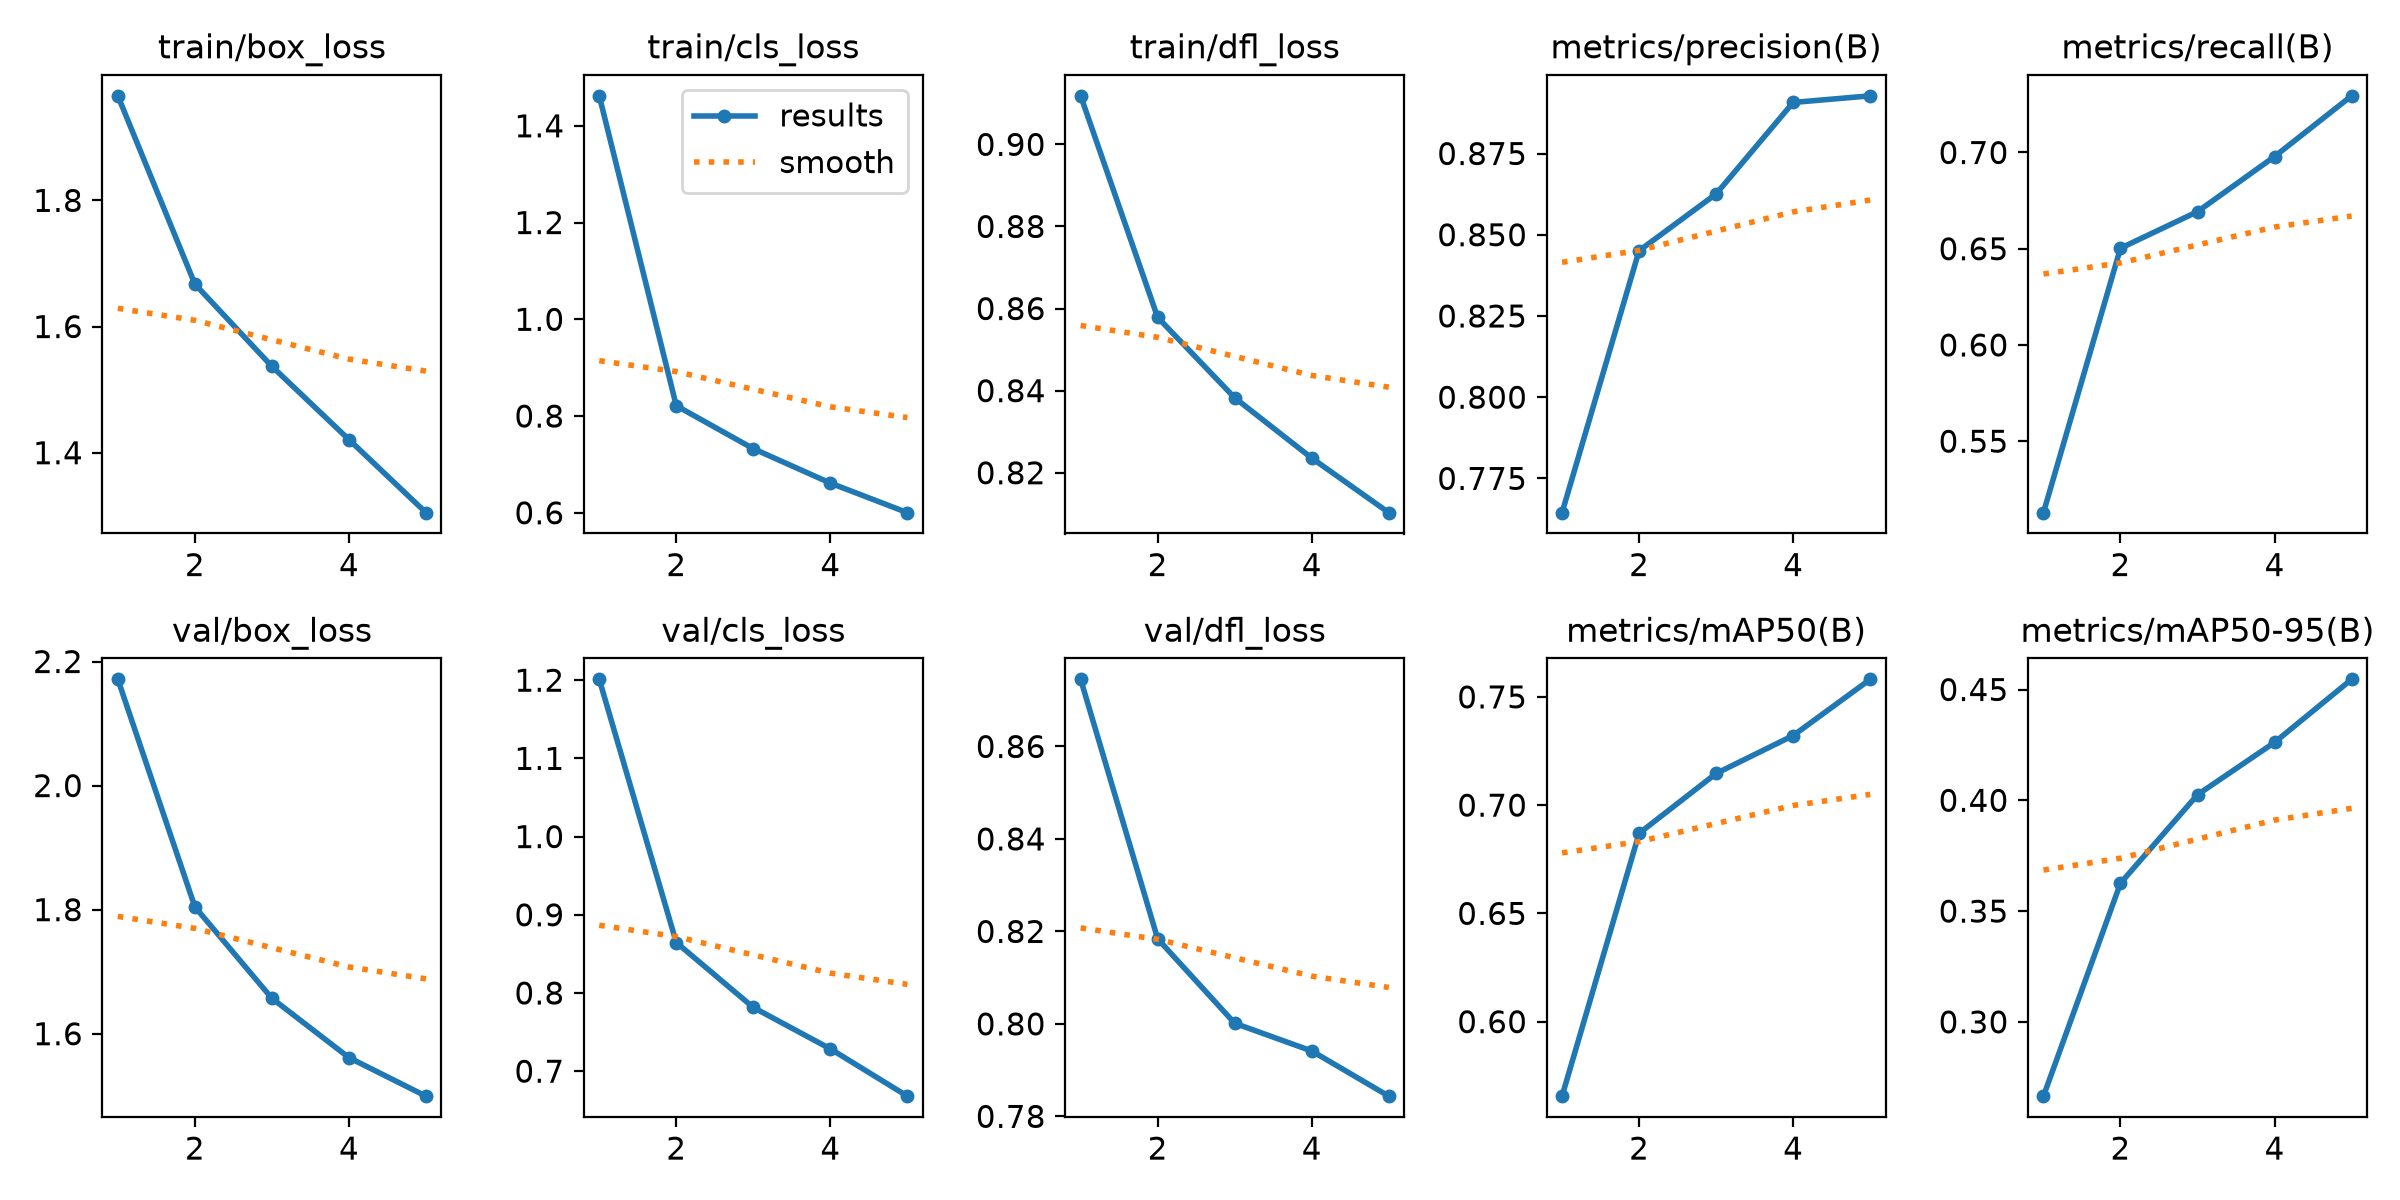
\includegraphics[width=\columnwidth]{lisa_training.png}
\caption{Curvas registradas para el entrenamiento YOLOv8n en LISA. Métricas de validación reportadas por época.}
\label{fig:lisa-curves}
\end{figure}

\begin{figure}[t]
\centering
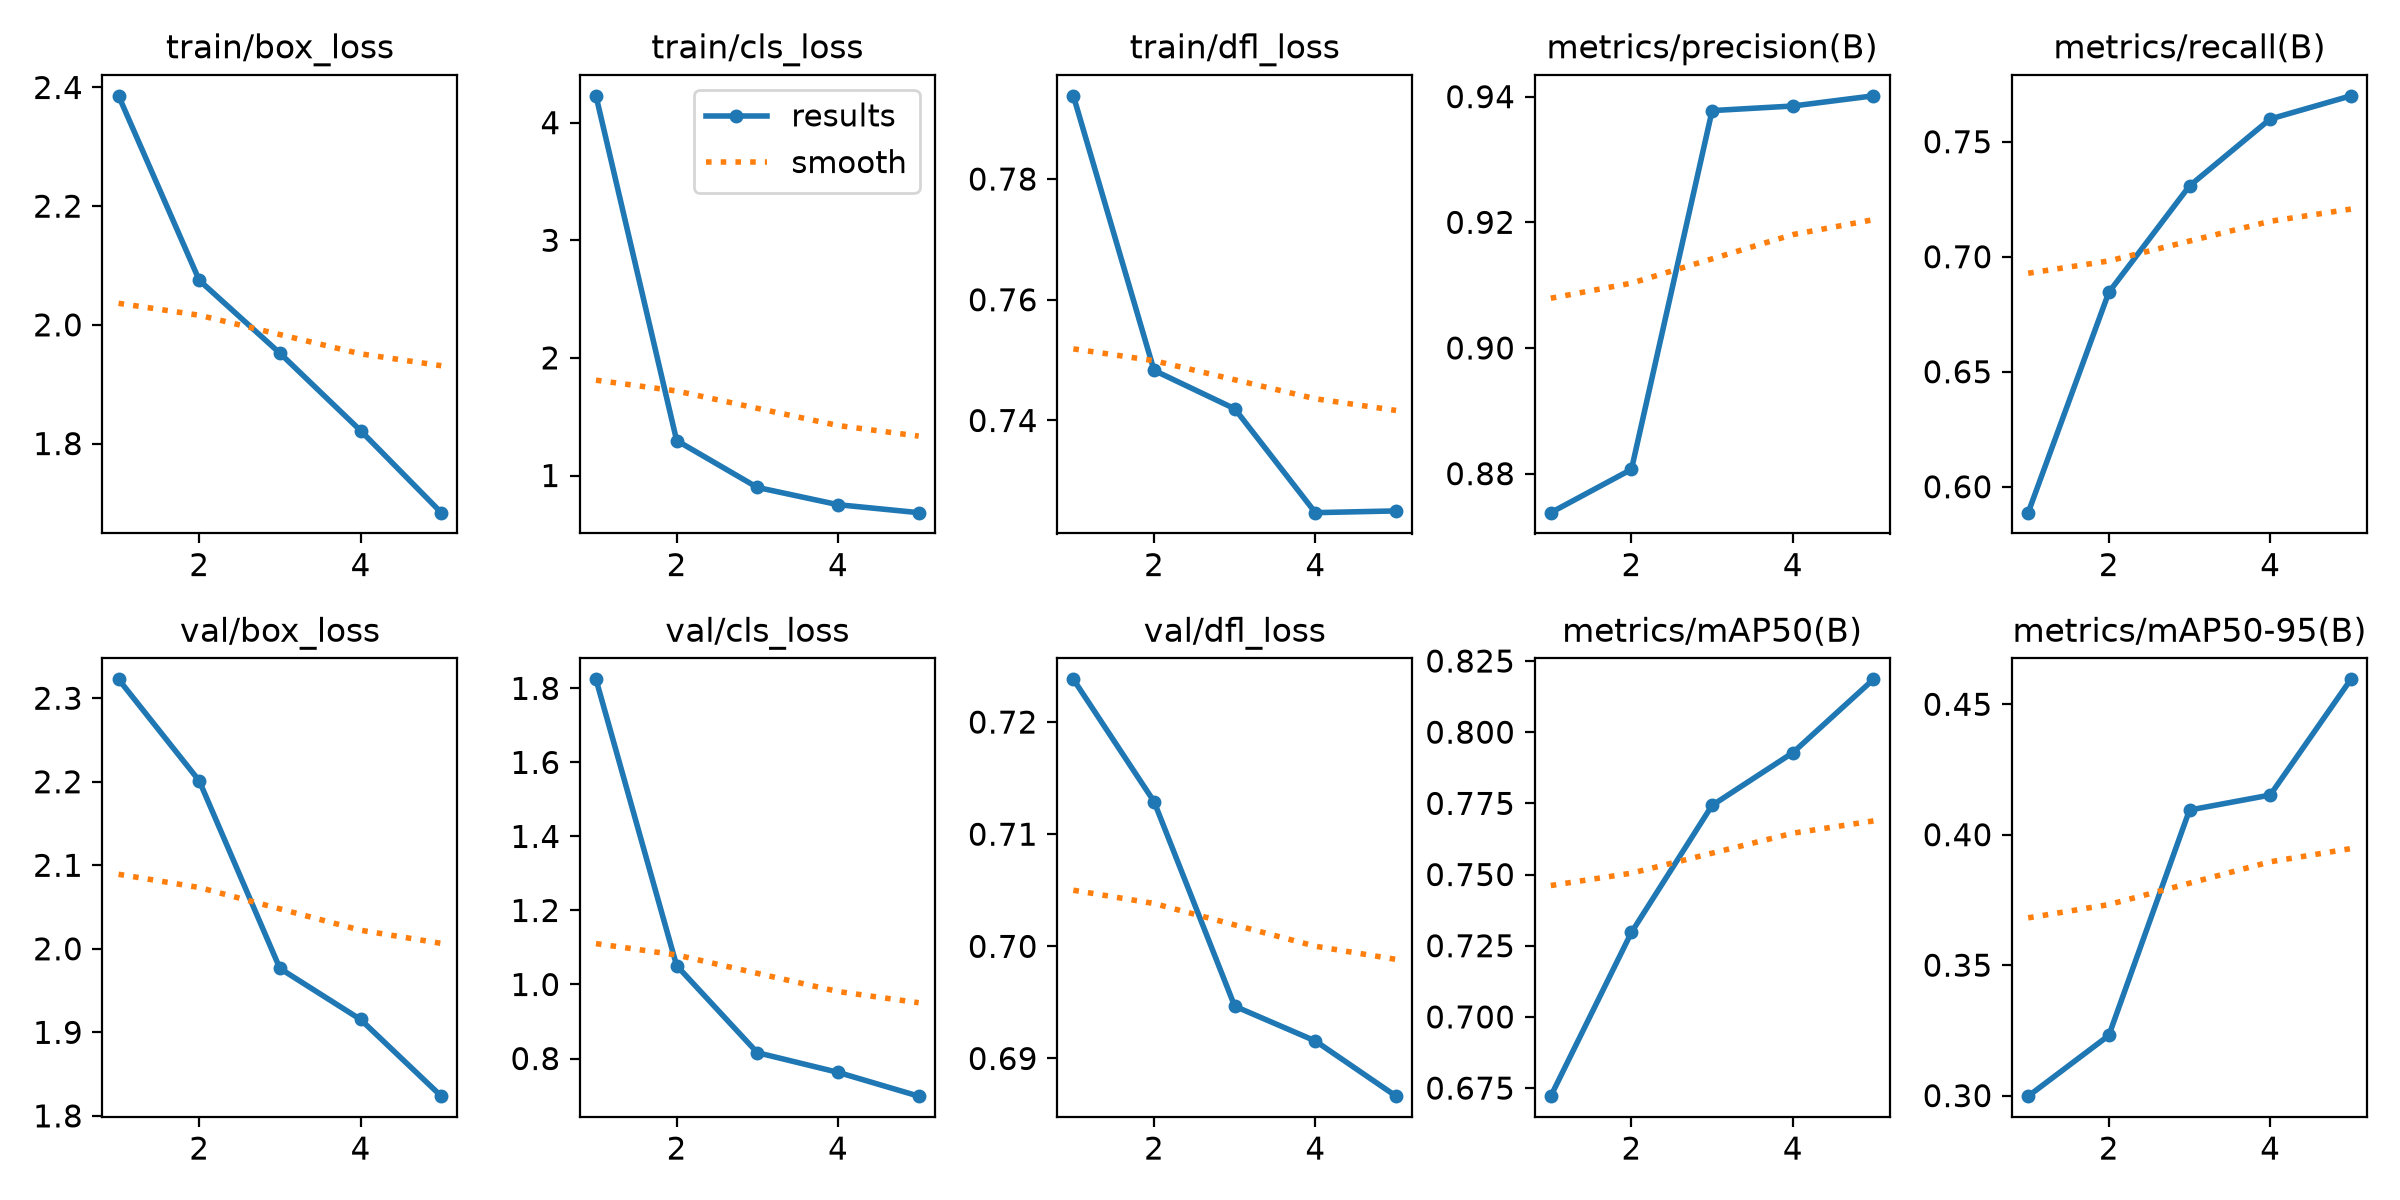
\includegraphics[width=\columnwidth]{bosch_training.png}
\caption{Curvas registradas para el entrenamiento YOLOv8n en Bosch BSTLD. Métricas de validación reportadas por época.}
\label{fig:bosch-curves}
\end{figure}

\begin{figure*}[t]
\centering
\begin{minipage}{0.48\textwidth}
  \centering
  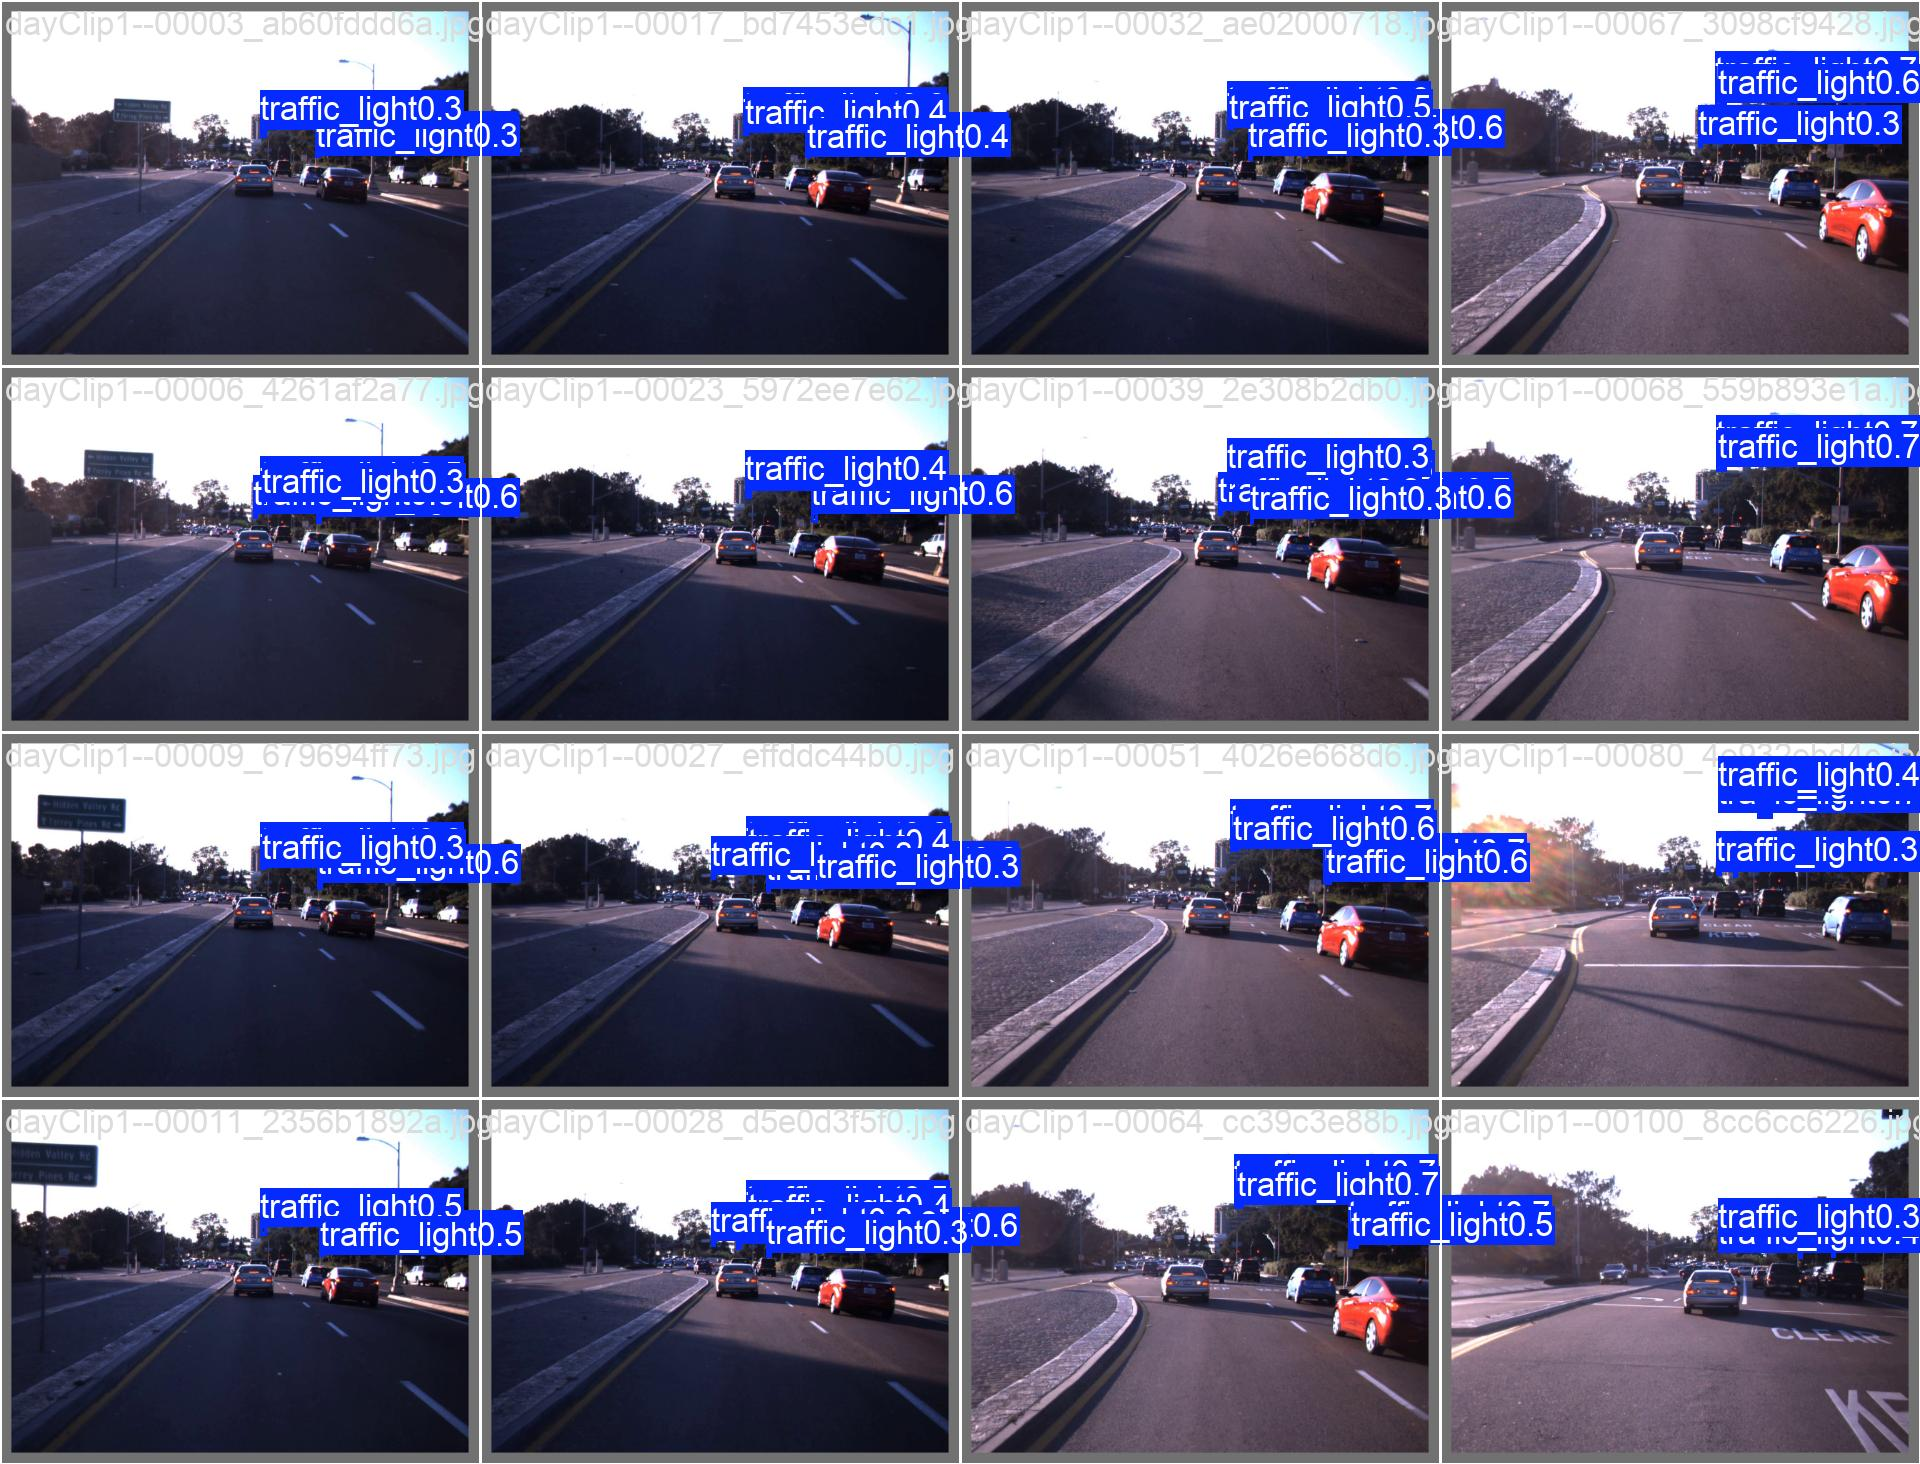
\includegraphics[width=\linewidth]{lisa_validation_predictions.jpg}\\[-1mm]
  (a) LISA
\end{minipage}\hfill
\begin{minipage}{0.48\textwidth}
  \centering
  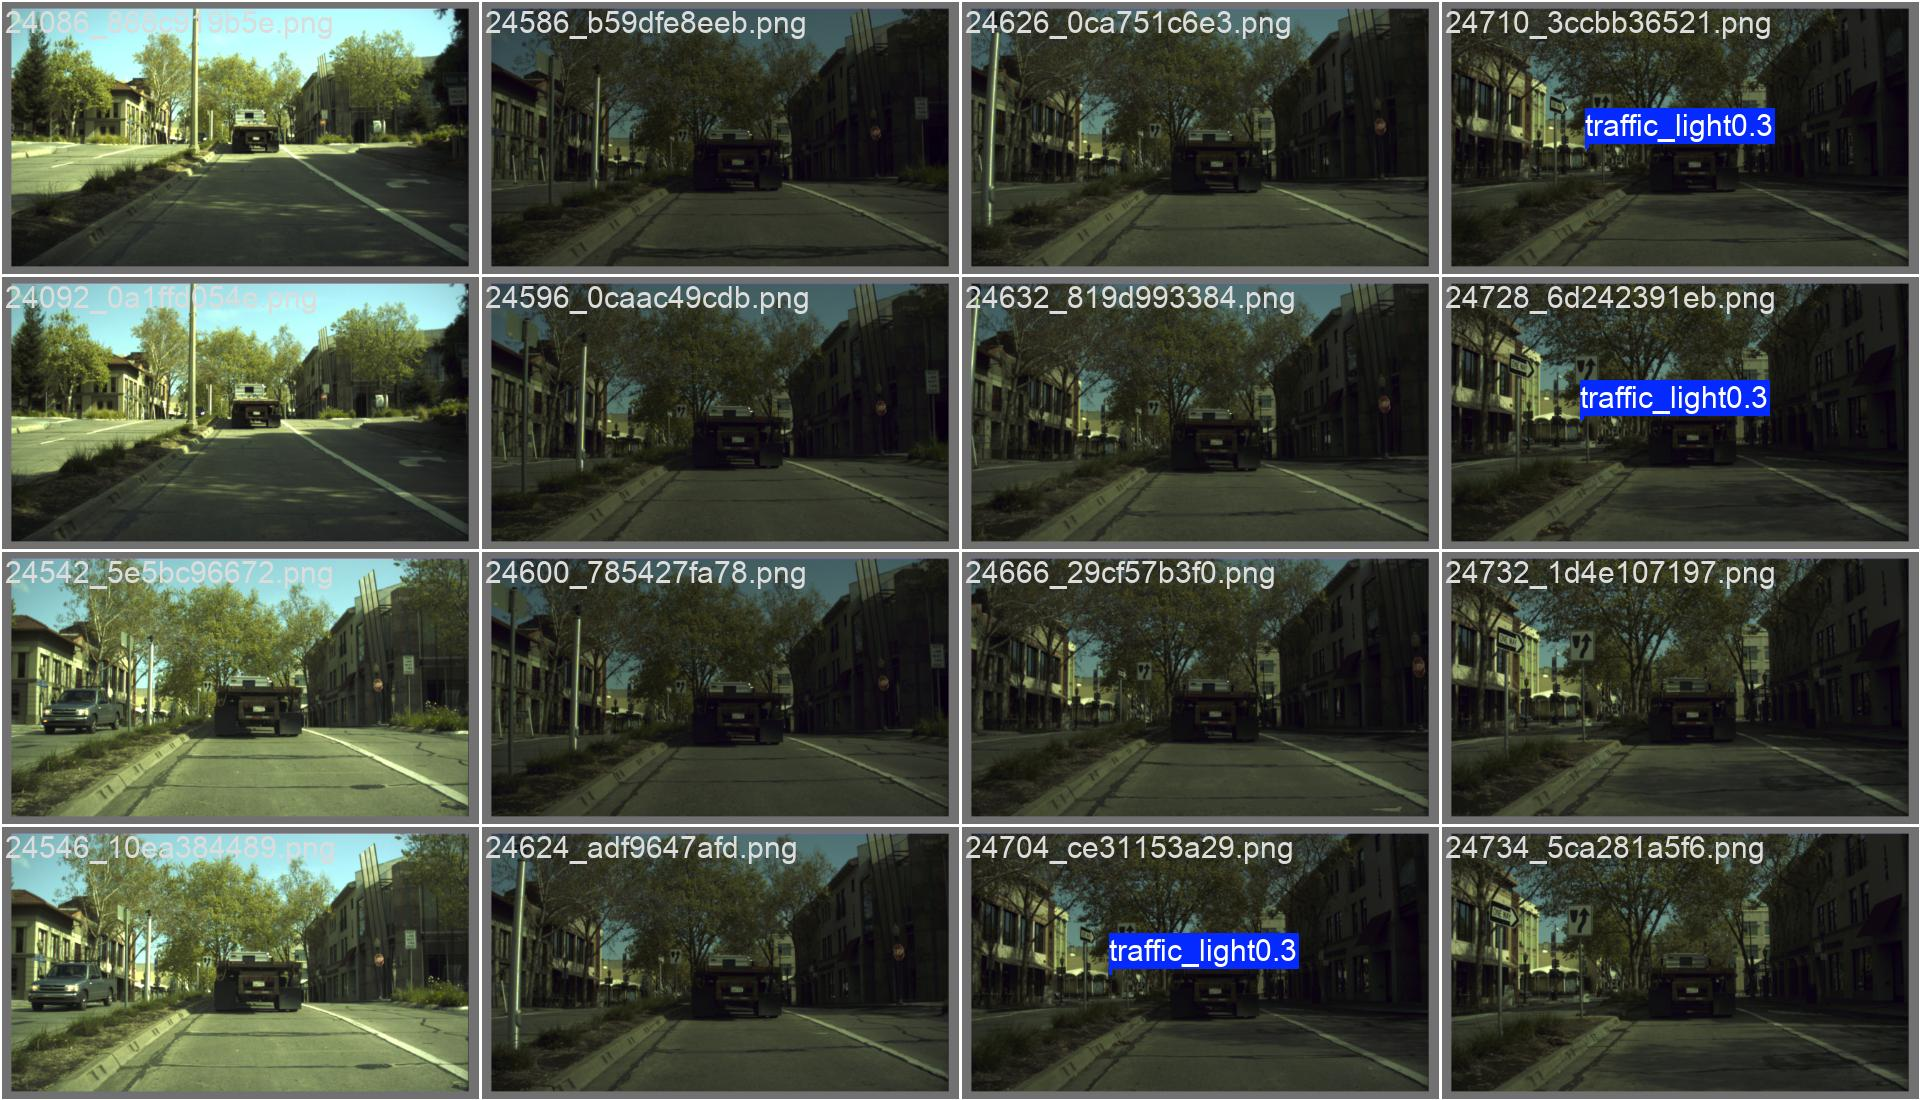
\includegraphics[width=\linewidth]{bosch_validation_predictions.jpg}\\[-1mm]
  (b) Bosch BSTLD
\end{minipage}
\caption{Mosaicos de predicciones guardados por Ultralytics para lotes de validación. Son visualizaciones de los datasets abiertos, no imágenes recolectadas por el equipo.}
\label{fig:predictions}
\end{figure*}

\subsection{Estado del código fuente}
El código Python no tiene todavía un pipeline de inferencia funcional: \texttt{backend/app/detector.py}, \texttt{classifier.py}, \texttt{state\_machine.py}, \texttt{camera.py}, \texttt{database.py} y \texttt{main.py} contienen actualmente comentarios de plantilla. Los ficheros de componentes Angular también son esqueletos con comentarios. Existen Dockerfiles y \texttt{docker-compose.yml}, pero el Compose actual es solo un comentario de plantilla. La carpeta \texttt{prototype/esp32/} solo contiene \texttt{.gitkeep}; \texttt{data/test\_videos/} tampoco contiene videos. En consecuencia, el repositorio acredita preparación de datos y entrenamiento por notebook, no la integración de cámara, detector en vivo, API, dashboard o banco físico.

El código público y los artefactos versionados pueden consultarse en el repositorio GitHub del proyecto \cite{repository}. Los datos raw y derivados locales se excluyen del control de versiones mediante reglas Git; su presencia local fue comprobada durante la preparación.

\section{Aporte diferencial e innovación}
La propuesta diferencia la detección genérica de semáforos de una futura inspección óptica externa orientada a verificar condiciones observables desde una cámara, sin conexión eléctrica al controlador. El avance concreto que respalda esta entrega es la ruta de datos local-first con respaldo de Drive, la conversión separada de anotaciones de dos fuentes y una línea base YOLO entrenada de forma independiente. La verificación de secuencia, diagnóstico de luminancia u obstrucción y validación física son hipótesis de desarrollo, no innovaciones ya demostradas. El aporte debe evaluarse frente a trabajos previos de detección, clasificación y seguimiento de semáforos \cite{jensen2016,behrendt2017,possatti2019,pavlitska2023}; no se afirma prioridad ni novedad científica comprobada.

\section{Limitaciones y trabajo pendiente}
Los experimentos disponibles son cortos (cinco épocas), usan un solo modelo base y no incluyen ablaciones, comparación con otras arquitecturas, evaluación cruzada entre fuentes, análisis de errores sistemático, latencia medida ni validación externa. La evaluación se hizo sobre \texttt{val}; reportar \texttt{test} después de finalizar selección y ajuste del modelo es necesario para una estimación final independiente. Las métricas no pueden compararse directamente con resultados publicados sin igualar datos, definición de clases, particiones y protocolo \cite{jensen2016,fernandez2018,pavlitska2023}.

El etiquetado unificado a una clase permite estudiar localización, pero elimina distinciones de color/estado y no sustenta aún detección de lente defectuoso. La división geométrica de una caja en tres lentes podría ser inadecuada para semáforos de distinta forma, orientación u oclusión; requiere implementación y validación. No se identificaron más de 100 imágenes propias ni videos o fallas controladas; deben recopilarse, etiquetarse y distinguirse de los datos públicos si la asignatura exige dicho componente.

Las siguientes tareas necesarias son: (1) entrenar con una duración justificada y seleccionar hiperparámetros sin usar el conjunto test; (2) evaluar los pesos finales una sola vez en test y documentar errores y latencia; (3) implementar y probar clasificación cromática y FSM con datos anotados de secuencias normales y anomalías; (4) obtener imágenes propias con autorización y procedencia documentada; (5) integrar módulos con la cámara, API y cliente web; y (6) realizar pruebas de sistema. La implementación física con ESP32 corresponde a una fase futura independiente.

\section{Conclusiones}
El estado actual de OptiSignal-AI es el de un prototipo algorítmico inicial: la preparación local de LISA y Bosch está ejecutada y validada, y existen dos modelos YOLOv8n entrenados de manera independiente durante cinco épocas, con métricas preliminares sobre validación. Los resultados justifican continuar investigando la localización de semáforos, pero no prueban la funcionalidad integral de inspección de fallas. El siguiente avance decisivo es completar una evaluación separada sobre test y desarrollar la clasificación de estado y lógica temporal con datos de prueba verificables.

\begin{thebibliography}{30}
\bibitem{jensen2016} M. B. Jensen, M. P. Philipsen, A. M\o gelmose, T. B. Moeslund, and M. M. Trivedi, ``Vision for looking at traffic lights: Issues, survey, and perspectives,'' \emph{IEEE Trans. Intell. Transp. Syst.}, vol. 17, no. 7, pp. 1800--1815, 2016, doi: 10.1109/TITS.2015.2509509.
\bibitem{philipsen2015} M. P. Philipsen, M. B. Jensen, A. M\o gelmose, T. B. Moeslund, and M. M. Trivedi, ``Traffic light detection: A learning algorithm and evaluations on challenging dataset,'' in \emph{Proc. IEEE ITSC}, 2015, pp. 2341--2345, doi: 10.1109/ITSC.2015.378.
\bibitem{behrendt2017} K. Behrendt, L. Novak, and R. Botros, ``A deep learning approach to traffic lights: Detection, tracking, and classification,'' in \emph{Proc. IEEE ICRA}, 2017, pp. 1370--1377, doi: 10.1109/ICRA.2017.7989163.
\bibitem{fernandez2018} C. Fern\'andez, C. Guindel, N.-O. Salscheider, and C. Stiller, ``A deep analysis of the existing datasets for traffic light state recognition,'' in \emph{Proc. IEEE ITSC}, 2018, pp. 248--254, doi: 10.1109/ITSC.2018.8569914.
\bibitem{jensen2017} M. B. Jensen, K. Nasrollahi, and T. B. Moeslund, ``Evaluating state-of-the-art object detector on challenging traffic light data,'' in \emph{Proc. IEEE CVPR Workshops}, 2017, pp. 9--15.
\bibitem{muller2018} J. M\"uller and K. Dietmayer, ``Detecting traffic lights by single shot detection,'' in \emph{Proc. IEEE ITSC}, 2018, pp. 266--273, doi: 10.1109/ITSC.2018.8569683.
\bibitem{weber2016} M. Weber, P. Wolf, and J. M. Z\"ollner, ``DeepTLR: A single deep convolutional network for detection and classification of traffic lights,'' in \emph{Proc. IEEE Intelligent Vehicles Symp.}, 2016, pp. 342--348, doi: 10.1109/IVS.2016.7535408.
\bibitem{weber2018} M. Weber, M. Huber, and J. M. Z\"ollner, ``HDTLR: A CNN based hierarchical detector for traffic lights,'' in \emph{Proc. IEEE ITSC}, 2018, pp. 255--260, doi: 10.1109/ITSC.2018.8569794.
\bibitem{lee2019} E. Lee and D. Kim, ``Accurate traffic light detection using deep neural network with focal regression loss,'' \emph{Image Vis. Comput.}, vol. 87, pp. 24--36, 2019, doi: 10.1016/j.imavis.2019.04.003.
\bibitem{john2014} V. John, K. Yoneda, B. Qi, Z. Liu, and S. Mita, ``Traffic light recognition in varying illumination using deep learning and saliency map,'' in \emph{Proc. IEEE ITSC}, 2014, pp. 2286--2291.
\bibitem{john2015} V. John, K. Yoneda, Z. Liu, and S. Mita, ``Saliency map generation by the convolutional neural network for real-time traffic light detection using template matching,'' \emph{IEEE Trans. Comput. Imaging}, vol. 1, no. 3, pp. 159--173, 2015, doi: 10.1109/TCI.2015.2480006.
\bibitem{omachi2009} M. Omachi and S. Omachi, ``Traffic light detection with color and edge information,'' in \emph{Proc. IEEE Int. Conf. Comput. Sci. Inf. Technol.}, 2009, pp. 635--638, doi: 10.1109/ICCSIT.2009.5234518.
\bibitem{moizumi2016} H. Moizumi, Y. Sugaya, M. Omachi, and S. Omachi, ``Traffic light detection considering color saturation using in-vehicle stereo camera,'' \emph{J. Inf. Process.}, vol. 24, no. 2, pp. 349--357, 2016, doi: 10.2197/ipsjjip.24.349.
\bibitem{gong2010} J. Gong, Y. Jiang, G. Xiong, C. Guan, G. Tao, and H. Chen, ``The recognition and tracking of traffic lights based on color segmentation and CAMSHIFT for intelligent vehicles,'' in \emph{Proc. IEEE Intelligent Vehicles Symp.}, 2010, pp. 431--435, doi: 10.1109/IVS.2010.5548083.
\bibitem{zhang2015} J. Zhang, S. Xie, and J. Liu, ``Traffic light detection and recognition for autonomous vehicles,'' \emph{J. China Univ. Posts Telecommun.}, vol. 22, no. 1, pp. 50--56, 2015, doi: 10.1016/S1005-8885(15)60624-0.
\bibitem{gao2020} F. Gao and C. Wang, ``Hybrid strategy for traffic light detection by combining classical and self-learning detectors,'' \emph{IET Intell. Transp. Syst.}, vol. 14, no. 7, pp. 735--741, 2020, doi: 10.1049/iet-its.2019.0782.
\bibitem{possatti2019} L. C. Possatti, R. Guidolini, V. B. Cardoso, R. F. Berriel, T. M. Paix\~ao, C. Badue, A. F. De Souza, and T. Oliveira-Santos, ``Traffic light recognition using deep learning and prior maps for autonomous cars,'' in \emph{Proc. Int. Joint Conf. Neural Netw.}, 2019, doi: 10.1109/IJCNN.2019.8851927.
\bibitem{wang2021} Q. Wang, Q. Zhang, X. Liang, Y. Wang, C. Zhou, and V. I. Mikulovich, ``Traffic lights detection and recognition method based on the improved YOLOv4 algorithm,'' \emph{Sensors}, vol. 22, no. 1, Art. no. 200, 2022, doi: 10.3390/s22010200.
\bibitem{chuang2023} C.-H. Chuang, C.-C. Lee, J.-H. Lo, and K.-C. Fan, ``Traffic light detection by integrating feature fusion and attention mechanism,'' \emph{Electronics}, vol. 12, no. 17, Art. no. 3727, 2023, doi: 10.3390/electronics12173727.
\bibitem{wang2023} X. Wang, J. Han, H. Xiang, B. Wang, G. Wang, H. Shi, L. Chen, and Q. Wang, ``A lightweight traffic lights detection and recognition method for mobile platform,'' \emph{Drones}, vol. 7, no. 5, Art. no. 293, 2023, doi: 10.3390/drones7050293.
\bibitem{lee2024} H.-Y. Lin and Y.-C. Chen, ``Traffic light detection using ensemble learning by boosting with color-based data augmentation,'' \emph{Int. J. Transp. Sci. Technol.}, 2024, doi: 10.1016/j.ijtst.2024.10.012.
\bibitem{trinci2026} T. Trinci, S. Magistri, T. Bianconcini, L. Taccari, L. Sarti, and F. Sambo, ``Color is not enough: Dataset and method for identifying relevant traffic lights in driving scenes,'' \emph{IEEE Trans. Intell. Transp. Syst.}, vol. 27, pp. 1116--1125, 2026, doi: 10.1109/TITS.2025.3626165.
\bibitem{redmon2016} J. Redmon, S. Divvala, R. Girshick, and A. Farhadi, ``You only look once: Unified, real-time object detection,'' in \emph{Proc. IEEE CVPR}, 2016, pp. 779--788.
\bibitem{liu2016} W. Liu et al., ``SSD: Single shot multibox detector,'' in \emph{Proc. Eur. Conf. Comput. Vis.}, 2016, pp. 21--37.
\bibitem{ren2015} S. Ren, K. He, R. Girshick, and J. Sun, ``Faster R-CNN: Towards real-time object detection with region proposal networks,'' in \emph{Adv. Neural Inf. Process. Syst.}, vol. 28, 2015.
\bibitem{lin2017} T.-Y. Lin, P. Goyal, R. Girshick, K. He, and P. Doll\'ar, ``Focal loss for dense object detection,'' in \emph{Proc. IEEE Int. Conf. Comput. Vis.}, 2017, pp. 2980--2988.
\bibitem{huang2017} J. Huang et al., ``Speed/accuracy trade-offs for modern convolutional object detectors,'' in \emph{Proc. IEEE CVPR}, 2017, pp. 3296--3305.
\bibitem{pavlitska2023} S. Pavlitska, N. Lambing, A. K. Bangaru, and J. M. Z\"ollner, ``Traffic light recognition using convolutional neural networks: A survey,'' in \emph{Proc. IEEE ITSC}, 2023, pp. 2790--2796, doi: 10.1109/ITSC57777.2023.10422041.
\bibitem{sarker2024} T. Sarker and X. Meng, ``Traffic signal detection and recognition algorithms for autonomous vehicles: A brief review,'' \emph{J. Transp. Eng. A: Syst.}, vol. 150, no. 10, 2024, doi: 10.1061/JTEPBS.TEENG-8056.
\bibitem{repository} N. Acevedo et al., ``OptiSignal-AI: código fuente del proyecto,'' GitHub repository, 2026. [Online]. Available: \url{https://github.com/n1cpac/optisignal-ai/}. Accessed: Sep. 27, 2026.
\bibitem{jocher2023} G. Jocher, A. Chaurasia, and J. Qiu, ``Ultralytics YOLOv8,'' software, 2023. [Online]. Available: \url{https://github.com/ultralytics/ultralytics}.
\bibitem{bstlddataset} K. Behrendt and L. Novak, ``Bosch Small Traffic Lights Dataset,'' dataset, 2017, doi: 10.5281/zenodo.12706046.
\end{thebibliography}

\end{document}
